\documentclass{article}

\usepackage{titlesec}
\newcommand{\sectionbreak}{\clearpage}

\usepackage{fancyhdr}
\pagestyle{fancy}
\lhead{Emanuel Casiano-Diaz}
\rhead{CSYS300: PoCS - Homework 04 - 09/28/2018}
\renewcommand{\headrulewidth}{0.4pt}
\renewcommand{\footrulewidth}{0.4pt}

\usepackage{amsmath}
\usepackage{amssymb}
\usepackage{bm}
\usepackage{pdfpages}

\usepackage{enumerate}% http://ctan.org/pkg/enumerate

\usepackage{hyperref}
\hypersetup{
    colorlinks=true,
    linkcolor=blue,
    filecolor=magenta,      
    urlcolor=cyan,
}

\usepackage{booktabs,float,siunitx}
%\usepackage[demo]{graphicx} % omit 'demo' option in real document

\begin{document}

\section{Exercise 1: Rich-Get-Richer Model}

My implementation can be found here: \url{https://github.com/ecasiano/PrinciplesOfComplexSystems/blob/master/HW04/Q01/rgr.py} \\

\hrule % just to indicate width of text block

\begin{figure}[H]

\begin{minipage}{0.47\textwidth}
    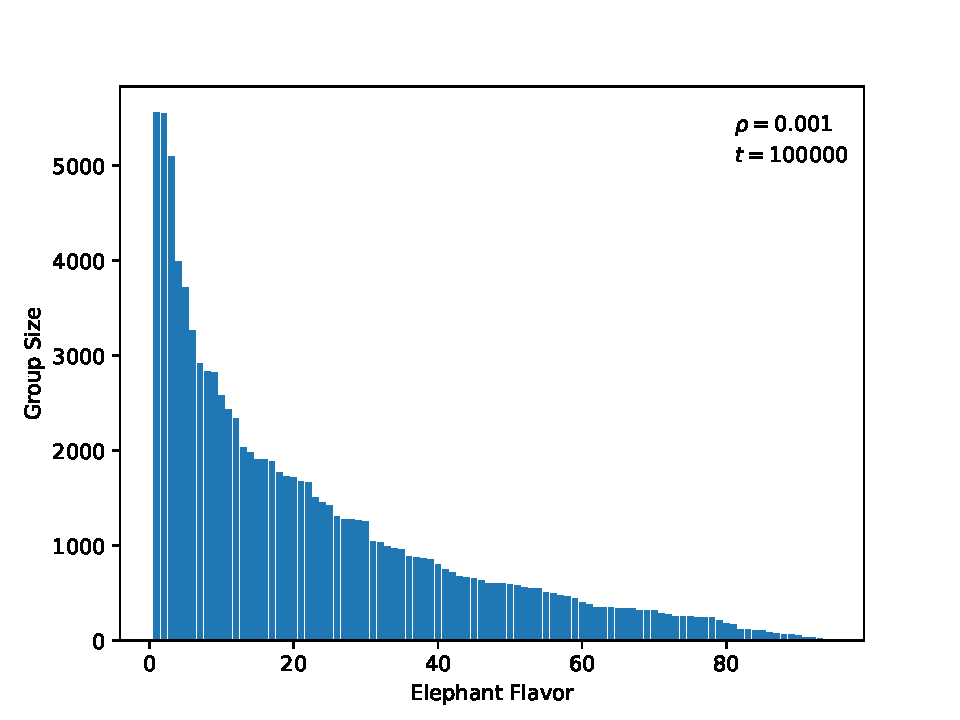
\includegraphics[width=\linewidth]{Q01/richGetRicherBarChart_rho0d001}
    \end{minipage}
    \hspace{\fill} % note: no blank line here
    \begin{minipage}{0.47\textwidth}
    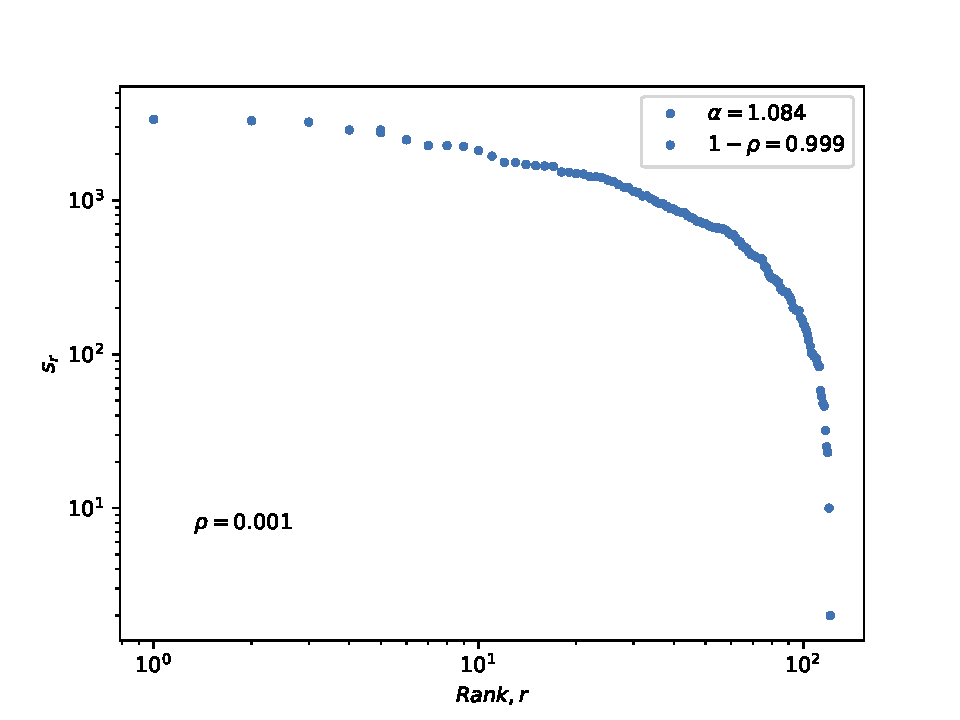
\includegraphics[width=\linewidth]{Q01/rgr_zipf_rho0d001.pdf}
    \end{minipage}

    \vspace*{0.20cm} % vertical separation

    \begin{minipage}{0.47\textwidth}
    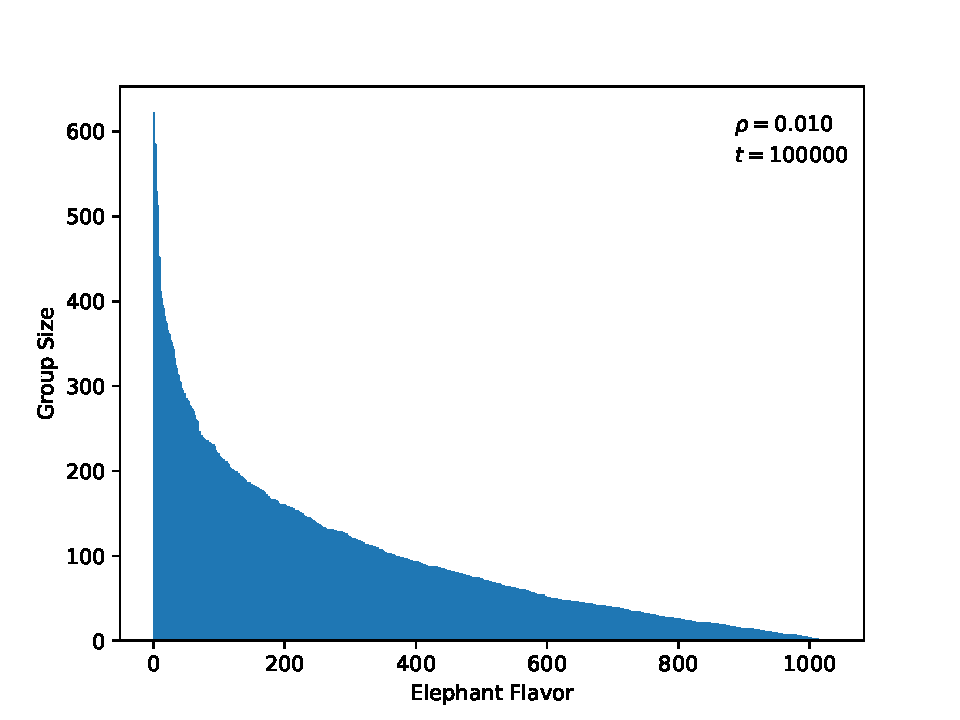
\includegraphics[width=\linewidth]{Q01/richGetRicherBarChart_rho0d010.pdf}
    \end{minipage}
    \hspace{\fill} % note: no blank line here
    \begin{minipage}{0.47\textwidth}
    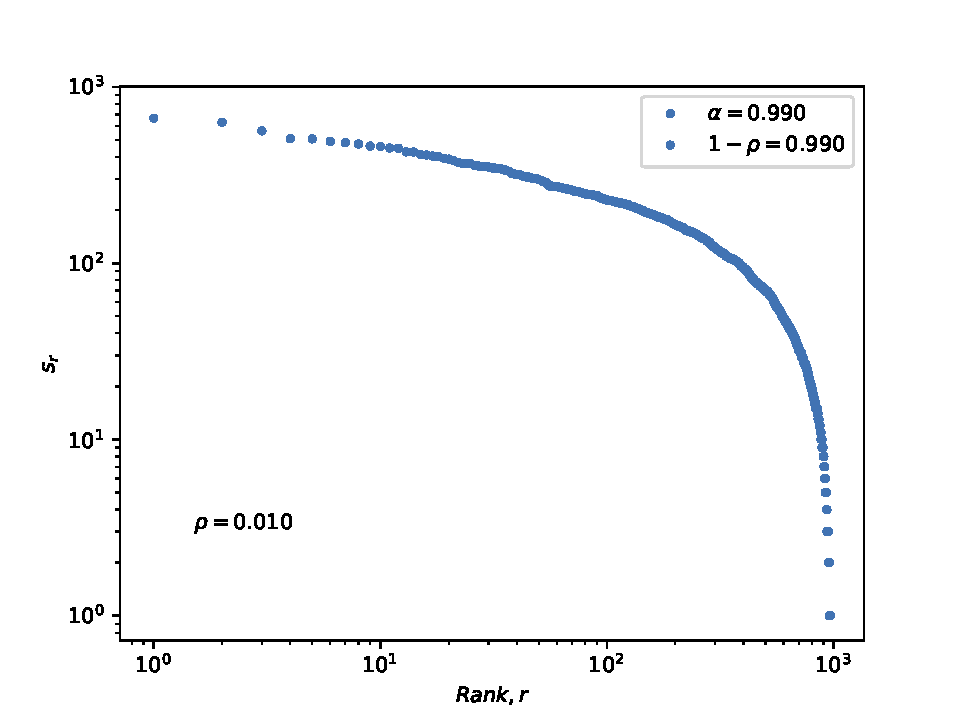
\includegraphics[width=\linewidth]{Q01/rgr_zipf_rho0d010.pdf}
    \end{minipage}
    
    \vspace*{0.20cm} % vertical separation
    
    \begin{minipage}{0.47\textwidth}
    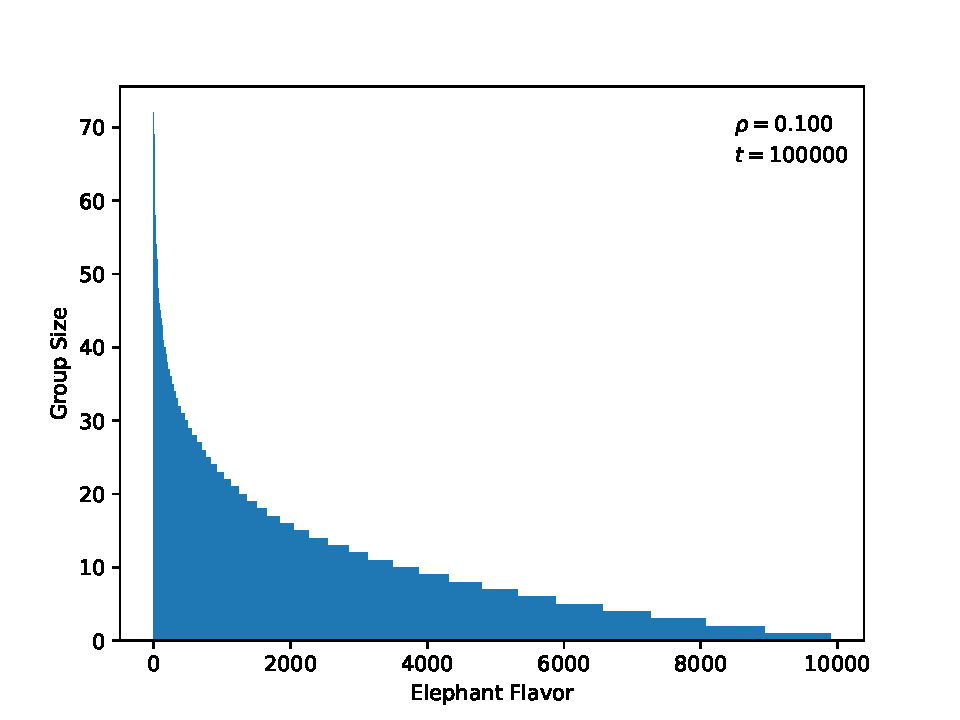
\includegraphics[width=\linewidth]{Q01/richGetRicherBarChart_rho0d100.pdf}
    \end{minipage}
    \hspace{\fill} % note: no blank line here
    \begin{minipage}{0.47\textwidth}
    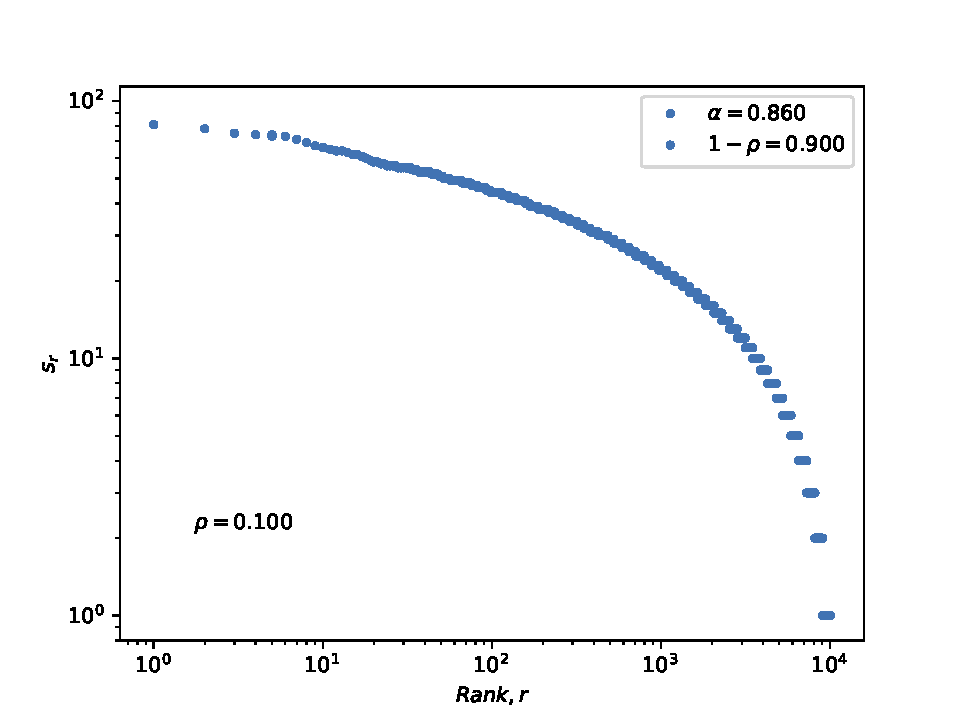
\includegraphics[width=\linewidth]{Q01/rgr_zipf_rho0d100}
    \end{minipage}
    
\caption{Left column: Sizes of each flavor group for various innovation rates, $\rho$. Notice that the number of groups is proportional to the innovation rate. Also, the richer groups for lower innovation rates are way more richer than their high innovation rate counterparts. Right column: Zipf distribution of group size vs rank for various innovation rates. The Zipfian exponent, $\alpha$, obtained from linear regression is compared to the difference $1-\rho$ and agreement between the two is seen.} \label{fig:4pics}
\end{figure}

\section{Exercise 2}

\subsection{a)} Let $n_k$ represent the normalized number of groups in the long time limit of the Random Competitive Replication (RCR) model is:

\[ \frac{n_k}{n_{k-1}} = \frac{(k-1)(1-\rho)}{1+(1-\rho)k}
\]

where $k\geq2$ is the group size and $\rho$ is the innovation rate. \\

The $n_1$ factor is given by $\rho-(1-\rho)n_1$, which in turn gives:

\[ n_1 = \frac{\rho}{2-\rho} \]


For simplicity, in the following discussion, the change of variables $(1-\rho) \equiv z$ will be employed. This will make $n_1 = \frac{1-z}{1+z}$. \\
 
The goal is to find an exact answer to the recursion $n_k$. The recursion can be expanded as:

\begin{align}
 n_k &= [\frac{z(k-1)}{1+zk}][\frac{z(k-2)}{1+z(k-1)}]\dots[\frac{z(2)}{1+z(3)}][\frac{z(1)}{1+z(2)}][\frac{1-z}{1+z}]  \\
 &= \frac{z^k(k-1)!(\frac{1}{z}-1)}{z^k[\frac{1}{z}+k][\frac{1}{z}+k-1]\dots[\frac{1}{z}+2][\frac{1}{z}+1]} \\
 &= \frac{(k-1)!(\frac{1}{z}-1)}{[\frac{(\frac{1}{z}+k)!}{(\frac{1}{z})!}]} \\
 n_k &= \frac{(k-1)!(\frac{1}{z})!}{(\frac{1}{z}+k)!} (\frac{1}{z}-1) 
\end{align}

Recall the definition of the Gamma and the Beta functions:

\[ \Gamma(k) = (k-1)!\]
\[ B(x,y) = \frac{\Gamma(x)\Gamma(y)}{\Gamma(x+y)}\]

In terms of these functions, the recursion becomes:

\[ n_k = (\frac{1}{z}-1) \frac{\Gamma(k) \Gamma(\frac{1}{z}+1)}{\Gamma(k+\frac{1}{z}+1)}  = (\frac{1}{z}-1) B(k,\frac{1}{z}+1)\]

where $z = 1-\rho$

\subsection{b)}

In the limit of large $k$, the Beta function goes as:

\[ B(k,\frac{1}{z}+1)  \sim k^{-(\frac{1}{z}+1)}\] \\

Replacing $z = 1-rho$ in the above definition, it is seen that the asymptotic behavior of $n_k$ is:

\[ n_k \sim k^{-(\frac{2-\rho}{1-\rho})}\] \\

Thus, the scaling exponent is:

\[ \gamma = \frac{2-\rho}{1-\rho} \]

where $0 \leq \rho \leq 1$.

\section{Exercise 3}

The above scaling will now be evaluating in the extreme cases of total innovation and total replication, or $\rho = 1$ and $\rho = 0$, respectively. \\

Case 1: Total innovation

\[ \lim_{\rho\to1} \gamma = \lim_{\rho\to1} \frac{2-\rho}{1-\rho} = \infty \] \\

This exponent implies that the number of groups with k elements will also be infinite. This makes sense since all of the elephants will be different and for large time steps, there will be an equally large number of groups. \\

Case 2: Total replication

\[ \lim_{\rho\to0} \gamma = \lim_{\rho\to0} \frac{2-\rho}{1-\rho} = 2 \]

This exponent implies that the number of groups with k elements will tend to 0. This makes sense since all of the elephants will form part of only the first group. Thus, there are no groups for large $k$ ($k\gg1$).

\section{Exercise 4: Fraction of k-sized groups}

\subsection{a)}

The fraction of $k$-sized groups at time $t$ is given by:

\[ n_k ^{(g)} = \frac{N_k(t)}{\rho t} = \frac{n_k t}{\rho t} = \frac{n_k}{t}\]

where $n_k$ is the exactly determined value obtained in Exercise 1:

\[ n_k = (\frac{\rho}{1-\rho}) B(k, \frac{2-\rho}{1-\rho})\]

Therefore the exact form of the fraction of $k$-sized groups is:

\[  n_k ^{(g)} = \frac{1}{t} [(\frac{\rho}{1-\rho}) B(k, \frac{2-\rho}{1-\rho}) ]\]

For $\rho \ll 1$, the following approximations are seen:

\[ n_1^{(g)} \sim B(1,2) \sim \frac{1}{2} \]
\[ n_2^{(g)} \sim B(2,2) \sim \frac{1}{6} \]
\[ n_3^{(g)} \sim B(3,2) \sim \frac{1}{12} \]

Notice how the fraction of rich groups is smaller than the fraction of poor groups!

\subsection{b)}

The estimated innovation rate for Joyce's "Ulysses" according to Simon is:

\[ \rho_{est} \approx 0.115 \]

Using the provided data, it is seen that this rate is instead slightly larger:

\[ \rho_{real} = \frac{\# \text{ of unique words}}{\# \text{ of total words}} \approx 0.119 \]

A relative error of 3.5\%. \\

The code used to evaluate the "Ulysses" corpus to determine the real innovation rate can be found here: \url{https://github.com/ecasiano/PrinciplesOfComplexSystems/blob/master/HW04/Q04/innovationRate.py}

\subsection{c)}

The fractions for $k=1,2,3$ sized groups in "Ulysses" was determined empirically using the code linked by calculating:

\[ n_k^{(g)} = \frac{\# \text{ of words with frequency k}}{\# \text{ of unique words}} \]

Using $\rho_{real} \approx 0.119$ and the forms from part a, the predicted fractions were calculated. Here is a summary of the predicted results: \\

\[ (n_1^{(g)})_{predicted} \approx 0.5316 , (n_1^{(g)})_{real} \approx 0.5649 \]
\[ (n_2^{(g)})_{predicted} \approx 0.1696, (n_2^{(g)})_{real} \approx 0.1556\]
\[ (n_3^{(g)})_{predicted} \approx 0.0820, (n_3^{(g)})_{real} \approx 0.0714\] 

Notice the good agreement between the results. The error slightly increases with group size. This is likely due to errors in the used data, since it will naturally be more inaccurate to count large group sizes.

\section{Exercise 5}

\subsection{a)} 

For brevity, I will pick up where the provided hint left off: \url{http://www.youtube.com/watch?v=4tqlEuXA7QQ}

\begin{align}
\sum_{k=mink_{max}}^{\infty} &= \frac{1}{N} \\
\sum_{k=mink_{max}}^{\infty} ck^{-\gamma} &= \frac{1}{N} \\
\implies  \sum_{k=mink_{max}}^{\infty} k^{-\gamma} &= \frac{1}{cN} \\
(mink_{max})^{-\gamma}  + \sum_{k=mink_{max}+1}^{\infty} k^{-\gamma} &= \frac{1}{cN}
\end{align}

In this last step, what I did was just write out the first term of the sum. Now, reindexing the sum in the second term of the left hand side such that it starts at $k = 0$, we get that:

\[ \sum_{mink_{max}+1}^{\infty} k^{-\gamma} = \sum_{k=0}^{\infty} [k+(mink_{max}+1)]^{-\gamma}  = \zeta(\gamma, (mink_{max}+1)) \]

where $\zeta(k+q) = \sum_{k=0}^{\infty} (k+q)^{-\gamma}$ for $Re(\gamma) > 1$ and $Re(q) > 0$ is the Hurwitz-Zeta function. Under the following conditions: $2 < \gamma < 3$ and $mink_{max} + 1 \geq 2$, the smallest and largest values of the $\zeta(\gamma,(mink_{max}+1))$ are 0 and 0.64, respectively. Thus, letting $\mathcal{Z} \equiv \zeta(\gamma,(mink_{max}+1))$ and solving for $mink_{max}$, it is seen that:

\[ mink_{max} = [\frac{1}{cN} - \mathcal{Z}]^{-1/\gamma} \]

where $0 < \mathcal{Z} < 0.64$

\subsection{b)}

\begin{align}
\langle k_{max} \rangle &= \sum_{k = mink_{max}}^{\infty} k P_k \\
&= (mink_{max}) P_{mink_{max}} + \sum_{k = mink_{max} + 1}^{\infty} k P_k \\
&= (mink_{max}) P_{mink_{max}} + \sum_{k = mink_{max} + 1}^{\infty} c k^{1-\gamma} \\
&= (mink_{max}) P_{mink_{max}} + \sum_{k = 0}^{\infty} c (k + mink_{max}+1)^{1-\gamma} \\
&= (mink_{max}) P_{mink_{max}} + \zeta(\gamma - 1, mink_{max}+1) \\
&=  [\frac{1}{cN} - \mathcal{Z}]^{-1/\gamma} c[  [\frac{1}{cN} - \mathcal{Z}]^{-1/\gamma} ] ^{-\gamma} + c \zeta(\gamma - 1, mink_{max}+1) \\
\langle k_{max} \rangle &=  [\frac{1}{cN} - \mathcal{Z}]^{\frac{-1}{\gamma} + 1} + c \zeta(\gamma - 1, mink_{max}+1)
\end{align}


\section{Exercise 6}

\subsection{a)}

The code used can be found here: \url{https://github.com/ecasiano/PrinciplesOfComplexSystems/tree/master/HW04/Q06}

\hrule % just to indicate width of text block

\begin{figure}[H]

\begin{minipage}{0.47\textwidth}
    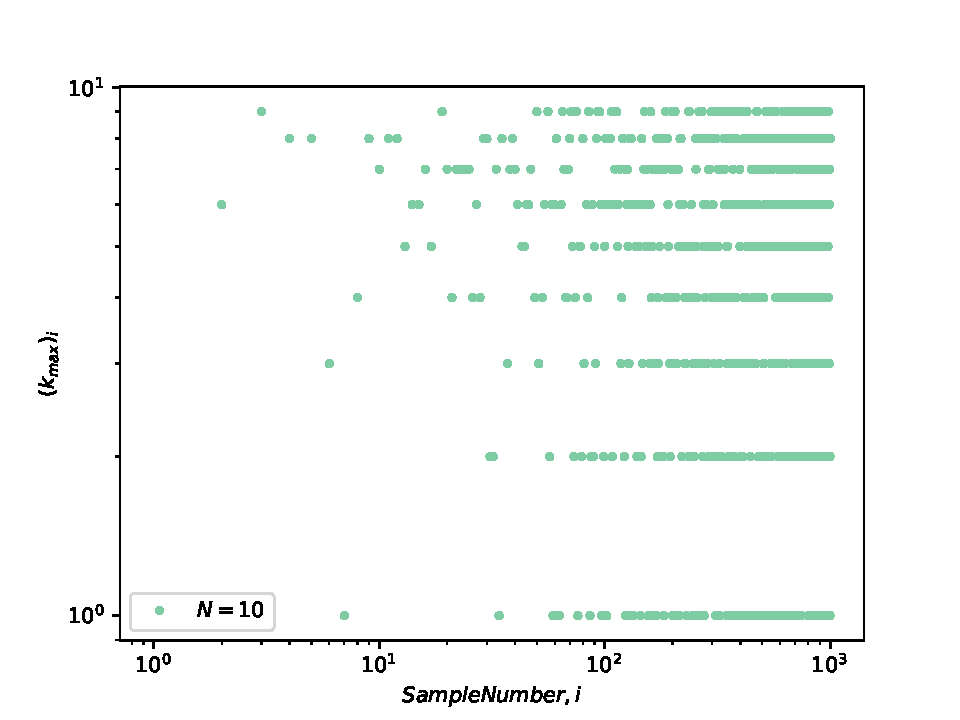
\includegraphics[width=\linewidth]{Q06/kmaxVsSampleNumber_N10.pdf}
    \end{minipage}
    \hspace{\fill} % note: no blank line here
    \begin{minipage}{0.47\textwidth}
    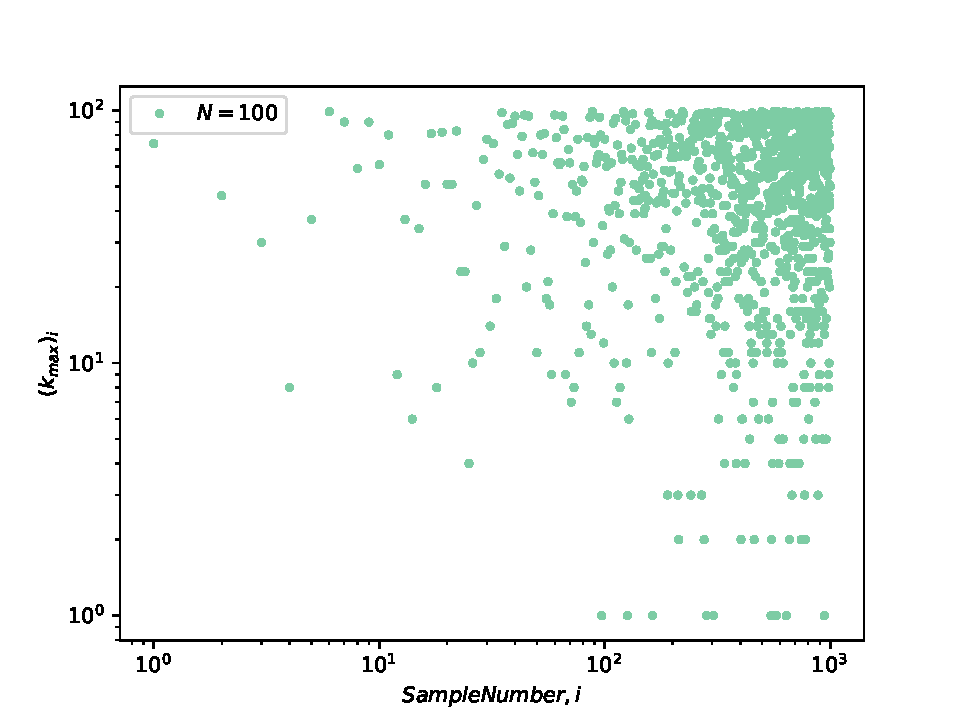
\includegraphics[width=\linewidth]{Q06/kmaxVsSampleNumber_N100.pdf}
    \end{minipage}

    \vspace*{0.20cm} % vertical separation

    \begin{minipage}{0.47\textwidth}
    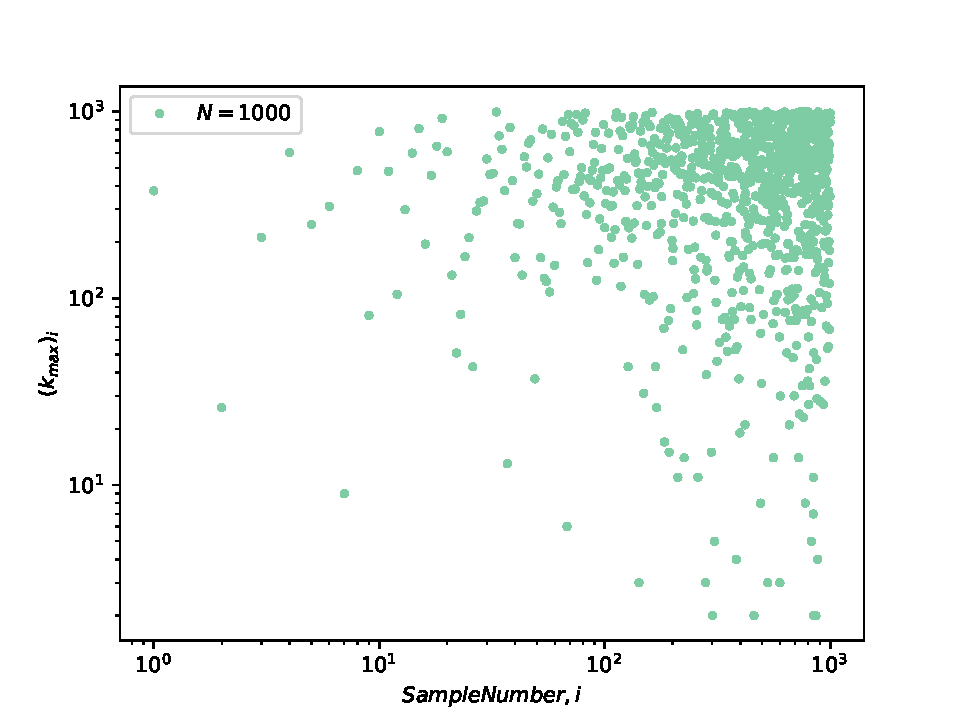
\includegraphics[width=\linewidth]{Q06/kmaxVsSampleNumber_N1000.pdf}
    \end{minipage}
    \hspace{\fill} % note: no blank line here
    \begin{minipage}{0.47\textwidth}
    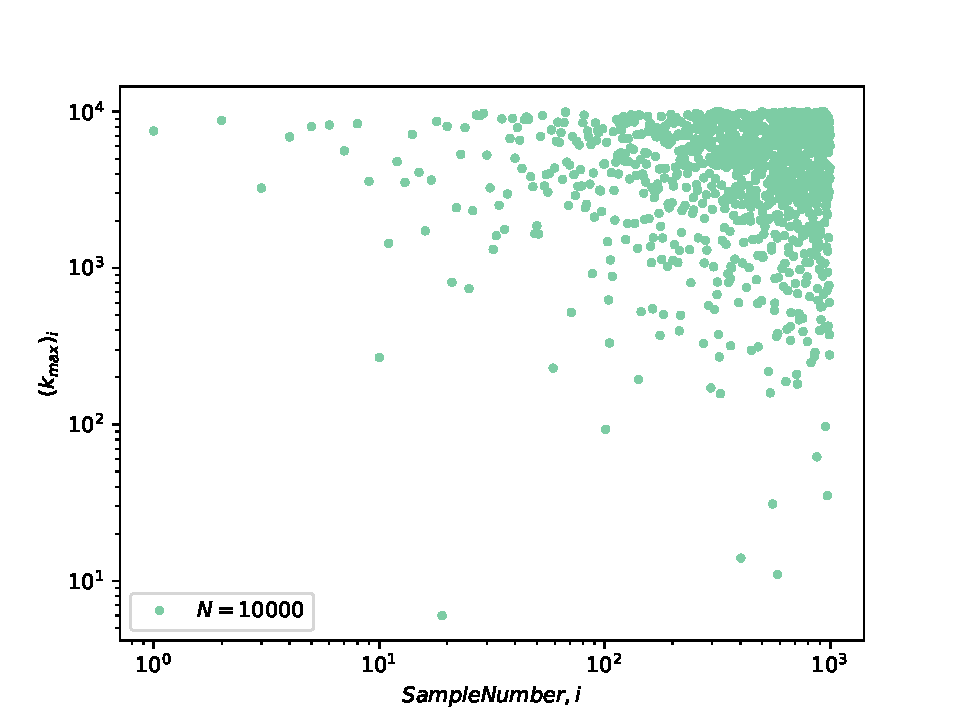
\includegraphics[width=\linewidth]{Q06/kmaxVsSampleNumber_N10000.pdf}
    \end{minipage}
    
    \vspace*{0.20cm} % vertical separation
    
    \begin{minipage}{0.47\textwidth}
    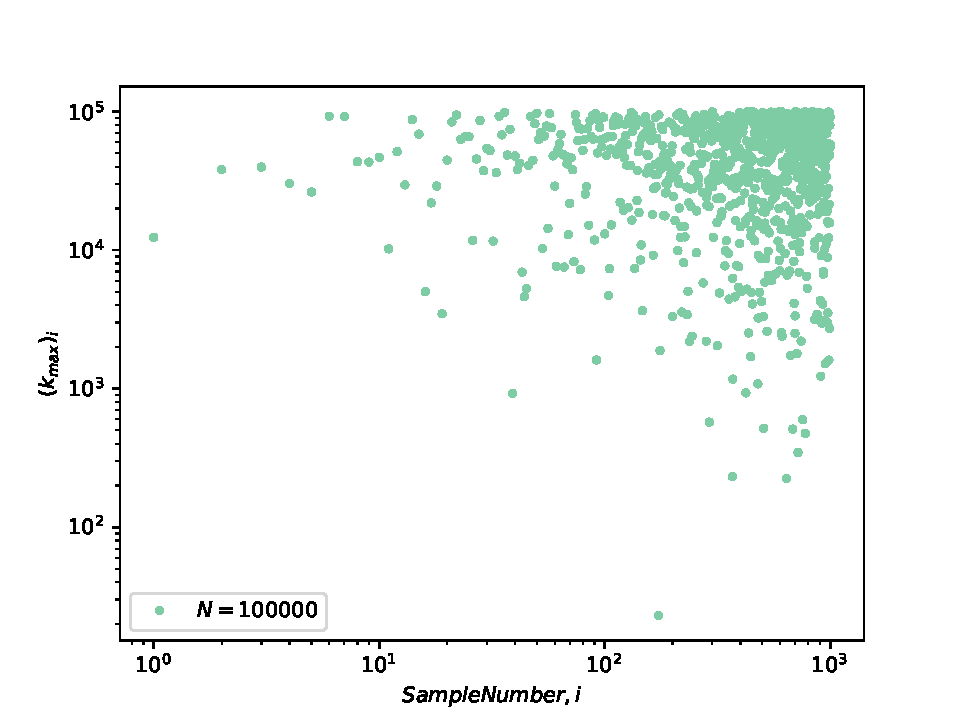
\includegraphics[width=\linewidth]{Q06/kmaxVsSampleNumber_N100000.pdf}
    \end{minipage}
    \hspace{\fill} % note: no blank line here
    \begin{minipage}{0.47\textwidth}
    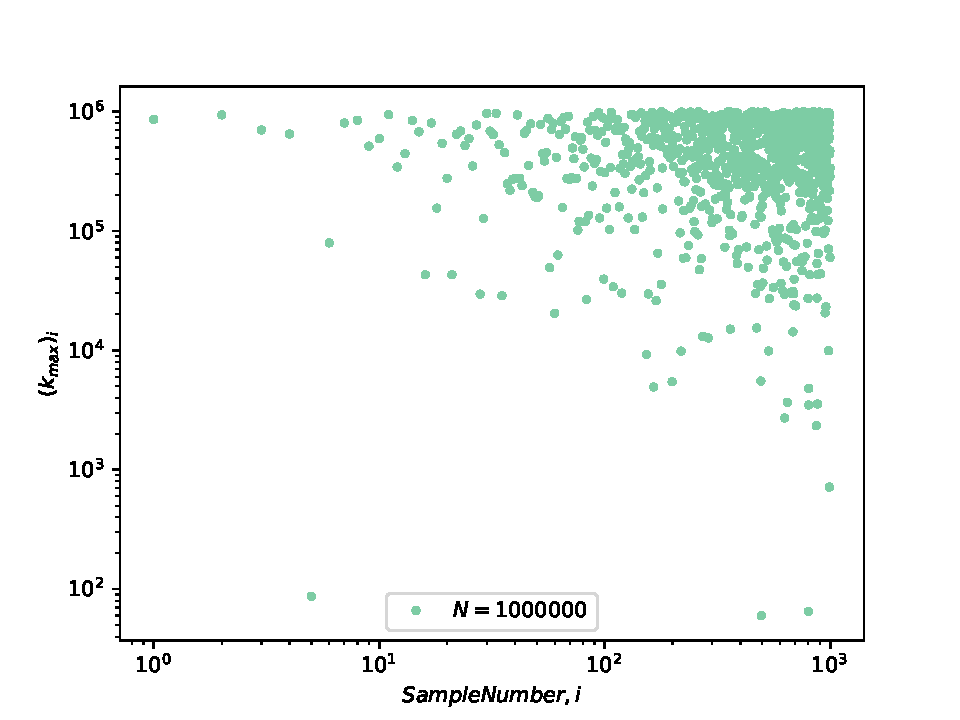
\includegraphics[width=\linewidth]{Q06/kmaxVsSampleNumber_N1000000.pdf}
    \end{minipage}
    
\caption{$k_{max}$ value for each of the $n=1000$ samples of a size $N$ set of random values distributed according to $P_k = \frac{k^{-5/2}}{\zeta(5/2)}$. Note the unevenness in $k_{max}$} \label{HeyJude}
\end{figure}

\subsection{b)}

\begin{figure}[h!]
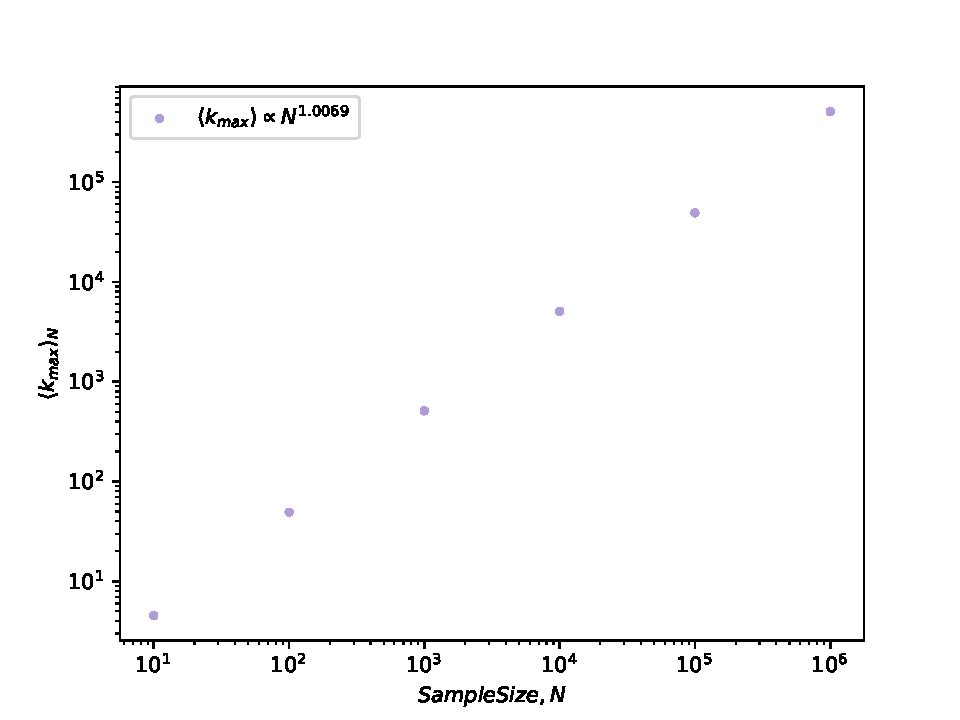
\includegraphics[width=\linewidth]{Q07/kmaxAverageVsSampleSize.pdf}
\caption{Average $k_{max}$ of each sample as a function of sample size $N$. The scaling goes almost perfectly as one. From the answers in the previous question, I would've expected a value closer to $0.70$ for the scaling. Perhaps the sums in that exercise had to be expanded more. Only the first term was used and the rest were neglected by assuming that they were a very small Hurwitz-Zeta function.}
\label{fig:envelope}
\end{figure}

\end{document}

\begin{figure}[h!]
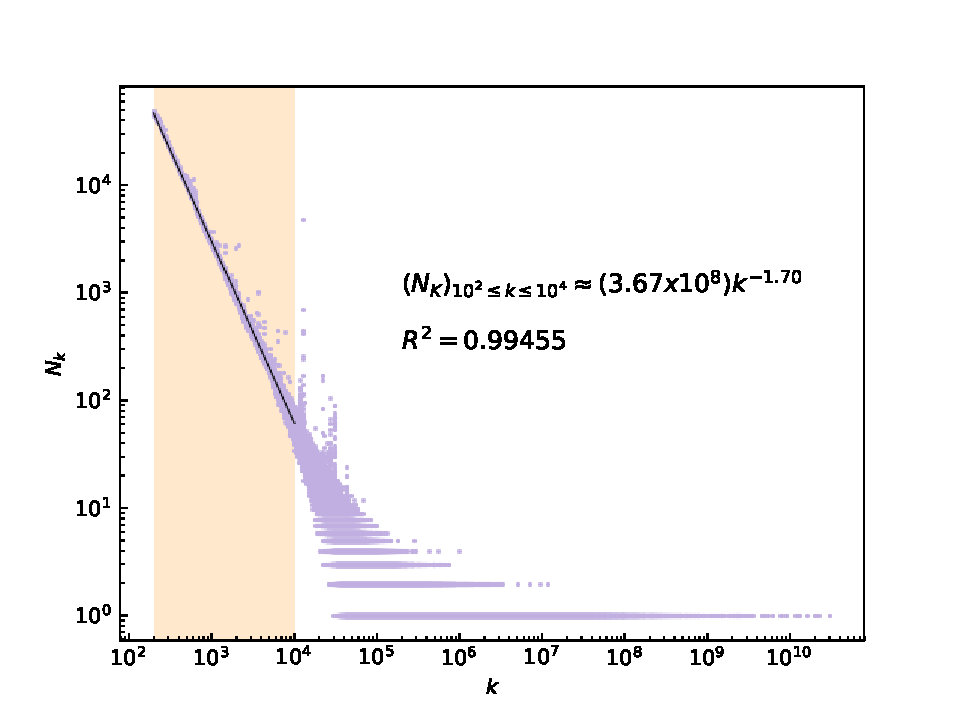
\includegraphics[width=\linewidth]{Q06/wordFrequencyLog.pdf}
\caption{Frequency $k$ that groups of $N_k$ words are repeated in a Google data set plotted in a base 10, log-log scale. The orange region denotes where power-law scaling holds (via "eye-balling"). By doing a linear regression on the sets $\log_{10} N_k$  ($y-$values) and $\log_{10} k$ ($x-$values) only inside the orange region, the prefactor and scaling exponent have been estimated to be $A \approx 3.67 x 10^{8}$ and $p \approx -1.70$, respectively.}
\label{fig:envelope}
\end{figure}